%%%%%%%%%%%%%%%%%%%%%%%%%%%%%%%%%%%%%%%%%%%%%%%%%%%%%%%%%%%%%%%%%%%%%%%%%%%%%%%%
% Template for USENIX papers.
%
% History:
%
% - TEMPLATE for Usenix papers, specifically to meet requirements of
%   USENIX '05. originally a template for producing IEEE-format
%   articles using LaTeX. written by Matthew Ward, CS Department,
%   Worcester Polytechnic Institute. adapted by David Beazley for his
%   excellent SWIG paper in Proceedings, Tcl 96. turned into a
%   smartass generic template by De Clarke, with thanks to both the
%   above pioneers. Use at your own risk. Complaints to /dev/null.
%   Make it two column with no page numbering, default is 10 point.
%
% - Munged by Fred Douglis <douglis@research.att.com> 10/97 to
%   separate the .sty file from the LaTeX source template, so that
%   people can more easily include the .sty file into an existing
%   document. Also changed to more closely follow the style guidelines
%   as represented by the Word sample file.
%
% - Note that since 2010, USENIX does not require endnotes. If you
%   want foot of page notes, don't include the endnotes package in the
%   usepackage command, below.
% - This version uses the latex2e styles, not the very ancient 2.09
%   stuff.
%
% - Updated July 2018: Text block size changed from 6.5" to 7"
%
% - Updated Dec 2018 for ATC'19:
%
%   * Revised text to pass HotCRP's auto-formatting check, with
%     hotcrp.settings.submission_form.body_font_size=10pt, and
%     hotcrp.settings.submission_form.line_height=12pt
%
%   * Switched from \endnote-s to \footnote-s to match Usenix's policy.
%
%   * \section* => \begin{abstract} ... \end{abstract}
%
%   * Make template self-contained in terms of bibtex entires, to allow
%     this file to be compiled. (And changing refs style to 'plain'.)
%
%   * Make template self-contained in terms of figures, to
%     allow this file to be compiled.
%
%   * Added packages for hyperref, embedding fonts, and improving
%     appearance.
%
%   * Removed outdated text.
%
%%%%%%%%%%%%%%%%%%%%%%%%%%%%%%%%%%%%%%%%%%%%%%%%%%%%%%%%%%%%%%%%%%%%%%%%%%%%%%%%

\documentclass[letterpaper,twocolumn,10pt]{article}
\usepackage{usenix2019_v3}

% to be able to draw some self-contained figs
\usepackage{tikz}
\usepackage{amsmath}
\usepackage{graphicx}
\apptocmd{\thebibliography}{\raggedright}{}{}
\graphicspath{ {./figures/} }

\begin{document}

%don't want date printed
\date{}

% make title bold and 14 pt font (Latex default is non-bold, 16 pt)
\title{\Large \bf Extending a File System to Support NVMe SSDs with SPDK}

%for single author (just remove % characters)
\author{
{\rm Ao Li}\\
University of Toronto
\and
{\rm Geoffrey Yu}\\
University of Toronto
} % end author

\maketitle

\thispagestyle{empty}
\begin{abstract}
Non-volatile memory express (NVMe) based solid state devices have undergone
tremendous innovation---leading to significant increases in performance.
However file systems have been slow to keep up; in many cases their design
(kernel space and lock based) impedes their ability to leverage the full
performance offered by NVMe storage devices. So how should next generation file
systems be designed to leverage the performance offered by NVMe storage
devices?

In this work we take a first step towards answering this question by extending
an existing user space file system to support NVMe storage devices by using
SPDK---a user space, polled, lockless device driver. We additionally modify 
the write path of the file system to support multi-threaded asynchronous I/O. The key
idea behind our design is to use a multi-threaded architecture to be able to
submit asynchronous I/O requests for different types of file system blocks
(e.g.  metadata versus data) in parallel.

Through experiments, we show that our multi-threaded asynchronous write
path is able to offer up to a $1.5\times$ improvement for single file writes
and up to a $3\times$ improvement for multi-file single transaction writes when
compared to a write path implemented with synchronous I/O.
\end{abstract}

\section{Introduction}
The emergence of the non-volatile memory express (NVMe)
specification~\cite{nvme} coupled with faster solid state storage devices
(SSDs) have together paved the way for new opportunities to improve the
performance of storage applications. In particular, the NVMe specification
introduces new avenues for parallelism by providing applications parallel
access to the underlying storage device through multiple I/O
queues~\cite{nvme}. File systems, a major storage application, are prime
candidates for these performance improvement opportunities.

Unfortunately, many file systems today are not designed to take advantage of
these opportunities. They
\begin{enumerate*}[label={(\roman*)}]
  \item reside in kernel space, requiring slow context switches to access;
  \item use locks to coordinate access to shared data, limiting their
    scalability; and
  \item are not written to take advantage of the parallelism exposed by NVMe.
\end{enumerate*}
So how should next generation file systems be designed to leverage the
performance improvements offered by NVMe storage devices?

In this work we take a first step towards answering this question by extending
an existing user space file system to support NVMe storage devices. We do this
with the goal of {\it quantifying} the potential performance benefit of
NVMe-designed file systems. Specifically, as a proof of concept, we integrate
testFS~\cite{testfs} (a toy user space file system) with SPDK~\cite{spdk} (a
user space lockless driver for NVMe devices) and we modify the file system's
write path to support multi-threaded asynchronous I/O.

The key idea in our design is to use a multi-threaded architecture to allow
different types of I/O requests to be submitted to and queued on the storage
device in parallel. This approach enables us to improve the performance of the
file system's write path by submitting asynchronous I/O requests for file
system metadata (e.g. inodes) and data in parallel by using different threads.

We benchmark our implementation and show that it can offer up to a $1.5\times$
improvement on single file writes and up to a $3\times$ improvement on
multi-file single transaction writes when compared to synchronous I/O.

\vspace{0.75em}
\noindent
In summary, our project makes the following contributions:
\begin{itemize}
  \item We propose a method to support multi-threaded asynchronous I/O on an
    NVMe SSD that can be implemented alongside existing synchronous code.
  \item We implement a proof of concept of our design by modifying the testFS
    write path and integrating it with with SPDK.
  \item We benchmark our implementation and show that our design offers up to a
    $1.5\times$ improvement for single file writes and up to a $3\times$
    improvement for multi-file single transaction writes when compared to
    synchronous I/O.
\end{itemize}

\section{Background}

In this section we present the background of NVMe interface and SPDK 
framework. We also present testFS, a user space file system that our 
file system is based on.

\subsection{NVMe and I/O Queue}

NVMe~\cite{nvme} is an open interface specification designed to allow host
software to communicate with a non-volatile memory subsystem (NVM) via a 
peripheral component interconnect express (PCIe) bus. Previous standards
such as serial-attacked SCSI and serial advanced technology attachment
can handle queue depths of 254 and 32 respectively. NVMe is able to 
handle queue depths of up to 65535 I/O queues with up to 64 Ki outstanding
commands per I/O queue, which allows an NVMe device to support parallel
operations. An I/O queue is composed of a submission queue and a completion
queue. Host software issues I/O commands to a submission queue and completions
are placed into the associated completion queue by the controller. Note that
the order of completions is not determined by the submission oder of the commands.

\subsection{SPDK and Block Devices}

SPDK~\cite{spdk} is an open source library that allows developer to implement
high performance, scalable, user-mode storage applications. A block device 
in SPDK is an abstraction of all block devices, where I/O commands are 
processed and issued to corresponding physical block devices such as NVMe 
devices and Malloc devices. SPDK provides a event framework, where  
different threads to exchange data through passing messages to one another.
It allows a user to build asynchronous, lockless, and high performance
applications.

\begin{figure}
  \centering
  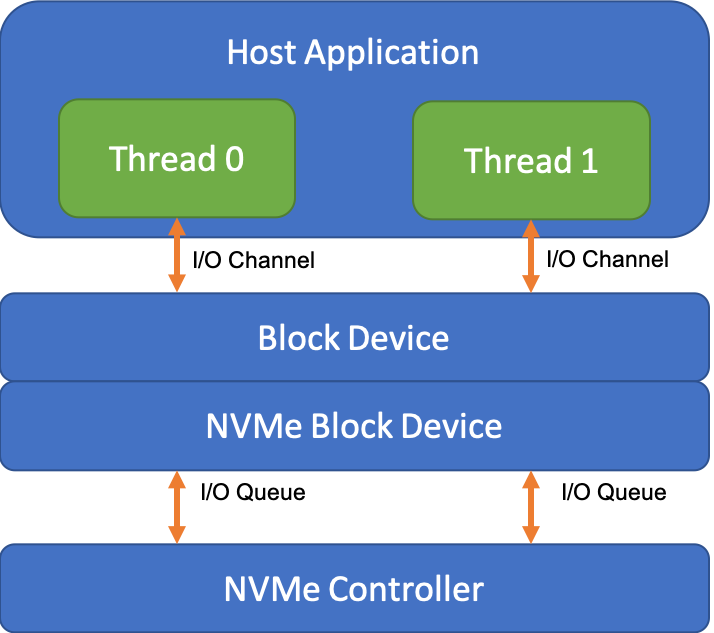
\includegraphics[height=6cm]{spdk_arch}
  \caption{Example of an SPDK application.}
  \label{fig:spdk_arch}
\end{figure}

For each thread, SPDK uses an io channel to represent the channel for accessing an 
I/O device. I/O requests issued to the block device will be forwarded to the underlying
physical device. In our implementation, io channel corresponds to I/O queue 
of the underlying NVMe device, the framework builds I/O commands based on I/O 
requests and submits them to submission queue. It then polls for I/O completion
on each queue pair with outstanding I/O to receive completion callbacks.  
Figure~\ref{fig:spdk_arch} provides a graphical
representation of a host application using SPDK block devices to interact with
an NVMe device. In the host application, each thread submit I/O requests to its
corresponding I/O channel and the I/O channel forward the I/O requests to the 
actual physical device based on the implementation of the physical block device.
The framework invokes the callback function when the I/O request is finished.

\subsection{TestFS}

TestFS\cite{testfs} is a user space file system which is similar to EXT3, a
journaled file system that is commonly used by the Linux kernel. TestFS
has three levels of indirections, which is illustrated in Figure~\ref{fig:testfs}.
A super block points to meta data and an inode block of the root directory. 
The meta data store the freemap of blocks as well as the checksum of the data blocks.
Inode blocks point to data blocks where the actual data are stored. In testFS, both 
directory data and indirect inode data are stored in data blocks. The
space for inode blocks and data blocks are pre-allocated and fixed during the
life cycle of testFS.

Note that our file system is based on testFS because testFS is well maintained, user
level, and well documented file system, that allows us to build a proof of concept
quickly. We believe our modifications to testFS can be applied to most of file systems.

\begin{figure}[h!]
  \centering
  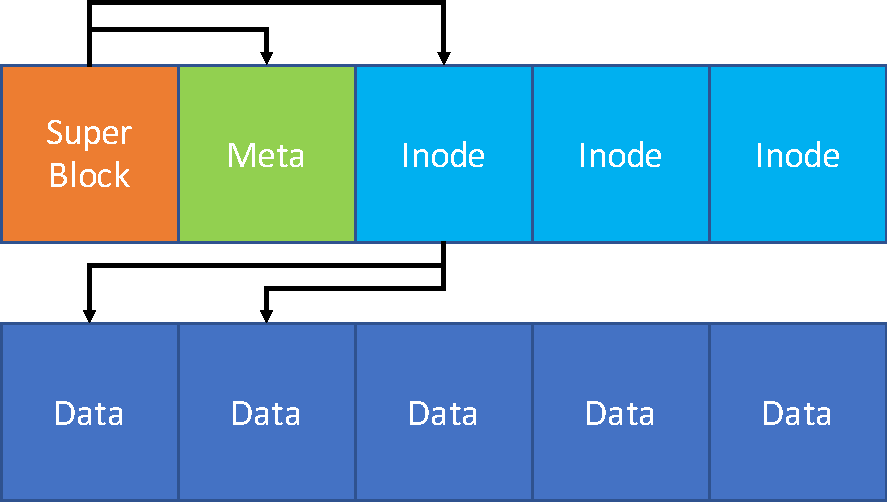
\includegraphics[height=3cm]{testfs}
  \caption{The layout of blocks with different types in testFS.}
  \label{fig:testfs}
\end{figure}

\section{Project Overview}
In this section we provide an overview of our project by enumerating our goals,
describing the primary challenges we faced, and highlighting the key ideas
behind our approach to addressing these challenges to meet our goals.

\subsection{Project Goals}
The high level goal of our project is to explore the feasibility and
performance implications of enabling parallel access to NVMe storage devices in
a user space file system. We work toward this goal by integrating SPDK with
testFS. More concretely, in our project we aim to:

\begin{enumerate}
  \item Demonstrate the feasibility of using SPDK to interact with NVMe devices
    in testFS.
  \item Modify the testFS write path to leverage the ability to make
    asynchronous block writes with multiple threads.
  \item Quantify the performance improvements of an asynchronous write path by
    benchmarking our implementation.
\end{enumerate}

\subsection{Key Challenges}

\paragraph{Challenge 1: Callbacks and Synchronous Code.}
Reads and writes to block devices with SPDK are asynchronous operations. SPDK
uses callback functions as the mechanism for scheduling code that should run
after an asynchronous operation has completed. However testFS is designed with
synchronous operations in mind. The file system code is written with the
assumption that, after a thread makes an I/O request, the thread will wait
until the request completes before executing any additional code. Ultimately,
this combination of synchronous code and a library that uses asynchronous
callbacks makes it difficult to integrate testFS with SPDK without making
invasive changes throughout the testFS codebase.

\paragraph{Challenge 2: Lock Contention.}
Our project is a proof of concept for next generation file systems that may use
hundreds of threads. To ensure the scalability of our ideas, we need to avoid
designs that have multiple threads acquiring the same locks to prevent
contention among the threads.

\subsection{Our Approach: Key Ideas}
The key idea behind our approach is to leverage a multi-threaded architecture
where each thread has a specific purpose. Specifically, we use three threads:
\begin{enumerate*}[label={(\roman*)}]
  \item a control thread responsible for executing the file system logic and
    for interacting with the user through the testFS REPL,
  \item a metadata thread responsible for submitting I/O requests for blocks
    that are used for file system metadata, and
  \item a data thread responsible for submitting I/O requests for data blocks.
\end{enumerate*}
This architecture allows us to achieve asynchronous writes with multiple
threads without incurring a significant engineering overhead.

\paragraph{Reconciling Callbacks and Synchronous Code.}
A multi-threaded architecture allows us to use existing thread synchronization
techniques as a way to be able to wait for asynchronous requests to complete.
The threads responsible for issuing I/O requests are distinct from the control
thread, which means callbacks only need to be registered on the lowest level
code responsible for issuing read/write requests with SPDK. When asynchronous
requests complete, the callback will execute on the I/O request thread and can
then ``signal'' the control thread as needed. We discuss two techniques for
thread synchronization in Section~\ref{sec:threadsync}. Ultimately this
approach allows us to avoid adding callback functions throughout the entire
testFS codebase and therefore allows us to avoid making invasive changes to the
file system.

\paragraph{Avoiding Lock Contention.}
To avoid lock contention, we use thread synchronization techniques that either
\begin{enumerate*}[label={(\roman*)}]
  \item do not require locks, or
  \item have a lock per thread, to prevent contention among I/O threads.
\end{enumerate*}
We discuss our proposed thread synchronization techniques in greater detail in
Section~\ref{sec:threadsync}.

\section{Implementation Details}
To implement asynchronous writes with multiple threads in testFS, we added
utilities to facilitate thread synchronization and we modified the file
system's write path to make it more amenable to asynchronous writes. For a
mapping of the key changes to the relevant source code files, please see
Appendix~\ref{apx:codewalkthrough}.

\subsection{Thread Synchronization}\label{sec:threadsync}
In our multi-threaded architecture, the control thread needs to be able to wait
for asynchronous I/O requests to complete. We accomplish this through thread
synchronization using shared objects: a primitive future or several
semaphores. We describe both approaches, however for the remainder of the
report we only reference the primitive future technique as both synchronization
techniques accomplish the same thing from a concurrency control standpoint.

\subsubsection{Primitive Futures}
TODO

\subsubsection{Semaphores}
TODO

\subsection{Asynchronous I/O}
To implement asynchronous I/O, we added asynchronous analogues of the {\tt
read\_blocks()} and {\tt write\_blocks()} functions called {\tt
read\_blocks\_async()} and {\tt write\_blocks\_async()}. These {\tt async}
functions accept the same arguments as their synchronous counterparts. However
callers of these {\tt async} functions also need to pass in a pointer to a
future and the thread ID on which the I/O request should be handled. This
allows the control thread to direct metadata block requests and data block
requests to distinct threads.

When these asynchronous read/write functions are called, the future's {\tt
expected\_count} for the handling thread is first incremented and then the
request is sent to the handling thread using SPDK's message passing library.
Upon receiving this message, the handling thread then submits the I/O request
to the underlying NVMe device using its dedicated I/O channel. When the request
completes, a callback is executed on the handling thread. The callback function
increments the future's {\tt count} for the handling thread to ``notify'' the
calling thread that the request has completed. Since the I/O request is
asynchronous, the calling thread is free to do other work while the I/O request
is being handled. When the calling thread needs to wait for the I/O request to
be completed it can call {\tt spin\_wait()} on the future.

To be able to compare asynchronous I/O requests and synchronous I/O
requests, we modified {\tt read\_blocks()} and {\tt write\_blocks()} so that
they can work with SPDK as well. These functions were implemented by calling
their asynchronous counterparts and then immediately waiting on the future.
This ensures that the I/O request completes before the function returns.

\subsection{Write Path Modifications}
\paragraph{Motivation.}
When we initially added asynchronous operations to file writes in testFS we
discovered a number of inefficiencies in the code that led to repeated reads
and writes of the same physical blocks. In the existing implementation:
\begin{enumerate*}[label={(\roman*)}]
  \item an entire bitmap block is flushed to the underlying device each time a
    single block is allocated;
  \item entire checksum blocks are flushed for each modified checksum;
  \item an entire inode block is flushed for each modified inode;
  \item inode indirect blocks are read, modified, and written to the underlying
    device for every block appended to the file.
\end{enumerate*}
Since a write transaction in testFS may consist of writing multiple blocks to
more than one file, issuing entire metadata block writes for each modified data
block results in unnecessary write amplification because a single metadata
block may contain metadata for multiple data blocks. We discovered that these
inefficiencies led to poor performance even in our asynchronous implementation.
This led us to reimplement the file write path in testFS.

\paragraph{Bulk Metadata Flushes.}
We made the observation that metadata such as block checksums, the data
block freemap, and ``opened'' inodes are cached in-memory. As a result, it is
unnecessary to flush modified metadata blocks to the underlying device each
time a new data block is appended to a file. We modified the file write
implementation to instead keep track of the dirty cached metadata blocks and
then flush them all together in bulk at the end of a transaction. This approach
ensured that a metadata block is written to the underlying device at most once
per transaction.

\paragraph{In-Memory Indirect Blocks.}
We reduced the number of extra reads and writes of an inode's indirect block by
keeping a copy of the indirect block in memory. The indirect block is loaded
into memory lazily (i.e. when it is first requested). This allows subsequent
reads and writes to the indirect block to be made to the copy stored in-memory.
The modified indirect block is flushed to the underlying device together with
the in-memory copy of the inode.

\section{Evaluation}
Since testFS is a toy file system, we did not run any end-to-end file system
benchmarks such as {\tt fio}, or Filebench~\cite{filebench-tarasov16}. As a
result, we do not make claims about performance improvements for real
workloads. Instead, the goal of our evaluation was to quantify the potential
performance benefit of adopting multi-threaded asynchronous I/O for NVMe
devices in production-ready user space file systems.

Overall our experiments show that our asynchronous I/O write path performs up
to $1.5\times$ better on single file writes and up to $3\times$ better on
multi-file writes compared to a synchronous I/O write path.

\subsection{Experimental Methodology}
\paragraph{Setup.}
We ran our experiments on a machine\footnote{We used {\tt mel-12}.} with a
14-core Intel Xeon 2.40 GHz CPU and 128 GB of memory. The machine was equipped
with two Seagate PLC Nytro 5000 NVMe SSDs. We used one of these SSDs, with a
capacity of 400 GB, in our experiments. Our code was linked with the version of
SPDK at git hash
\href{https://github.com/spdk/spdk/commit/a2bf3cded37b7cc7e402eae80da90891f921b56d}{\tt a2bf3cded}.
We used a fixed block size of 512 bytes when interacting with the SSD.

\paragraph{Methodology.}
In each experiment we measured the amount of time it took to complete a given
task up to a granularity of microseconds. We repeated each experiment five
times and used the average of all five trials in our results. We used primitive
futures (described in Section~\ref{sec:futures}) as the thread synchronization
mechanism in all of our experiments.

\paragraph{Baseline.}
We wanted to quantify the performance improvement associated with using
multi-threaded asynchronous I/O on the testFS file write path. Therefore
our baseline was a synchronous version of the testFS write path (each
asynchronous I/O function call was replaced with its synchronous counterpart).
For a fair comparison, both the synchronous and asynchronous write paths used
our improved write path implementation (as described in
Section~\ref{sec:writepath}).

\begin{figure}
  \centering
  % Raw read/write sequential speedups
\begin{tikzpicture}[baseline]
\begin{axis}[
  xlabel=Number of Blocks,
  ylabel=Speedup,
  height=5cm,
  width=8cm,
  every axis plot/.append style={ultra thick},
  legend style={font=\footnotesize,at={(0.97,0.5)},anchor=east},
]
\addlegendimage{darkestblue, mark=none}
\addlegendimage{lightblue, mark=none}
%
\addplot [
  darkestblue,
  mark=none,
] table [
  x=num_blocks,
  y expr=\thisrow{sync_avg_us} / \thisrow{async_avg_us},
  col sep=comma,
] {data/raw_seq_read.csv};
%
\addplot [
  lightblue,
  mark=none,
] table [
  x=num_blocks,
  y expr=\thisrow{sync_avg_us} / \thisrow{async_avg_us},
  col sep=comma,
] {data/raw_seq_write.csv};
%
% Legend
\addlegendentry{Sequential Reads}
\addlegendentry{Sequential Writes}
\end{axis}
\end{tikzpicture}

  \caption{The speedup of asynchronous I/O versus synchronous I/O for
    sequential reads and writes of a varying number of blocks.}
  \label{fig:raw-speedup}
\end{figure}

\subsection{Raw Sequential Reads and Writes}
To quantify the raw performance of asynchronous I/O versus synchronous I/O, we
ran two microbenchmarks that read and write a sequence of blocks one by one.
In each trial the benchmark reads (or writes) one block in a loop for a
pre-determined number of iterations. In the synchronous case each read/write
blocks until the request completes. In the asynchronous case we issue all
read/write requests and then wait for them to complete together in bulk.

Figure~\ref{fig:raw-speedup} shows our results. As the number of blocks read or
written increases, the speedup increases. Additionally the read speedup (up to
$7\times$) is greater than the write speedup (up to $2\times$). Reads are
faster than writes in flash-based SSDs, which could mean that they benefit more
from asynchronous I/O; this would explain the discrepancy in speedups between
raw reads and writes.

\begin{figure*}
\centering
\begin{subfigure}[t]{0.49\linewidth}
  % Single File Async Writes - Speedup
\begin{tikzpicture}[baseline]
\begin{axis}[
  xlabel=Number of Blocks,
  ylabel=Speedup,
  height=4.5cm,
  width=8.5cm,
  every axis plot/.append style={ultra thick},
]
%
\addplot [
  darkestblue,
  mark=none,
  mark options={fill=darkestblue},
] table [
  x=num_blocks,
  y expr=\thisrow{sync_avg_us} / \thisrow{async_avg_us},
  col sep=comma,
] {data/e2e_write_num_blocks.csv};
%
\end{axis}
\end{tikzpicture}

  \caption{Single file write speedup}\label{fig:single-file-speedup}
\end{subfigure}\hfill%
\begin{subfigure}[t]{0.49\linewidth}
  % Single File Async Writes - Throughput
\begin{tikzpicture}[baseline]
\begin{axis}[
  xlabel=Number of Blocks,
  ylabel=Throughput (KiB/s),
  height=5cm,
  width=8.5cm,
  every axis plot/.append style={ultra thick},
  legend pos=south east,
  legend style={font=\footnotesize},
]
\addlegendimage{darkestblue, mark=none}
\addlegendimage{lightblue, mark=none}
%
\addplot [
  darkestblue,
  mark=none,
  mark options={fill=darkestblue},
] table [
  x=num_blocks,
  y expr={(0.5 * \thisrow{num_blocks}) / (\thisrow{async_avg_us} / 1000000)},
  col sep=comma,
] {data/e2e_write_num_blocks.csv};
%
\addplot [
  lightblue,
  mark=none,
  mark options={fill=lightblue},
] table [
  x=num_blocks,
  y expr={(0.5 * \thisrow{num_blocks}) / (\thisrow{sync_avg_us} / 1000000)},
  col sep=comma,
] {data/e2e_write_num_blocks.csv};
% Legend
\addlegendentry{Async. I/O}
\addlegendentry{Sync. I/O}
\end{axis}
\end{tikzpicture}

  \caption{Single file write effective throughput}\label{fig:single-file-thpt}
\end{subfigure}
\par\bigskip
\begin{subfigure}[t]{0.49\linewidth}
  % Multi File Async Writes - Speedup
\begin{tikzpicture}[baseline]
\begin{axis}[
  xlabel=Number of Files,
  ylabel=Speedup,
  height=4.5cm,
  width=8.5cm,
  every axis plot/.append style={ultra thick},
  legend pos=south east,
  legend style={font=\footnotesize},
]
\addlegendimage{darkestblue, mark=none}
\addlegendimage{lightblue, mark=none}
%
\addplot [
  darkestblue,
  mark=none,
] table [
  x=num_files,
  y expr=\thisrow{sync_avg_us} / \thisrow{async_avg_us},
  col sep=comma,
] {data/e2e_write_num_files_100bl.csv};
%
\addplot [
  lightblue,
  mark=none,
] table [
  x=num_files,
  y expr=\thisrow{sync_avg_us} / \thisrow{async_avg_us},
  col sep=comma,
] {data/e2e_write_num_files_10bl.csv};
%
% Legend
\addlegendentry{100 Data Blocks}
\addlegendentry{10 Data Blocks}
\end{axis}
\end{tikzpicture}

  \caption{Multi-file write speedup}\label{fig:multi-file-speedup}
\end{subfigure}%
\begin{subfigure}[t]{0.49\linewidth}
  % Multi-File Async Writes - Throughput
\begin{tikzpicture}[baseline]
\begin{axis}[
  xlabel=Number of Files,
  ylabel=Throughput (KiB/s),
  height=4.5cm,
  width=8.5cm,
  every axis plot/.append style={ultra thick},
  legend style={font=\footnotesize,at={(0.97,0.4)},anchor=east},
]
\addlegendimage{darkestblue, mark=none}
\addlegendimage{lightblue, mark=none}
%
\addplot [
  darkestblue,
  mark=none,
  mark options={fill=darkestblue},
] table [
  x=num_files,
  y expr={(0.5 * 100 * \thisrow{num_files}) / (\thisrow{async_avg_us} / 1000000)},
  col sep=comma,
] {data/e2e_write_num_files_100bl.csv};
%
\addplot [
  lightblue,
  mark=none,
  mark options={fill=lightblue},
] table [
  x=num_files,
  y expr={(0.5 * 100 * \thisrow{num_files}) / (\thisrow{sync_avg_us} / 1000000)},
  col sep=comma,
] {data/e2e_write_num_files_100bl.csv};
% Legend
\addlegendentry{Async. I/O}
\addlegendentry{Sync. I/O}
\end{axis}
\end{tikzpicture}

  \caption{Multi-file write effective throughput for 100 data blocks}
  \label{fig:multi-file-thpt}
\end{subfigure}
\caption{The speedup and effective write throughput when appending a varying
number of data blocks to a single file and when appending a fixed number of
blocks to a varying number of files.}
\end{figure*}

\subsection{File Writes}
To quantify the performance improvements associated with multi-threaded
asynchronous I/O we ran experiments that varied the number of blocks written to
a file and the number of files written in a single transaction. In these
experiments we report the speedup and the effective write throughput, which is
calculated by dividing the total size of the data blocks being written by the
time taken to complete the experiment. Note that the effective write throughput
excludes I/O requests made to read and write file system metadata.

\subsubsection{Single File Writes}
In this experiment we measured the time taken to append a varying number of
data blocks to a single file in testFS. Figure~\ref{fig:single-file-thpt} shows
the effective write throughput when multi-threaded asynchronous I/O is used and
when synchronous I/O is used. Figure~\ref{fig:single-file-speedup} summarizes
this comparison by illustrating the speedup as the number of blocks being
appended increases.

The speedup improves as the number of blocks being appended increases. We think
this is attributed to two reasons:
\begin{enumerate*}[label={(\roman*)}]
  \item a larger number of blocks being queued allows the device to operate
    closer to its peak throughput, and
  \item the cost of reading and writing the file system metadata is amortized
    across a larger number of blocks.
\end{enumerate*}
Overall this experiment shows that our multi-threaded asynchronous write path
can offer up to a $1.5\times$ performance improvement over synchronous I/O for
single file writes.

\subsubsection{Multi-file Writes}
In this experiment we measured the time taken to append a fixed number of data
blocks to a varying number of files within a single transaction. In each trial
we opened all the files (i.e. loaded the corresponding inodes), made the writes
to each file, and then flushed all of the dirty metadata blocks at once in bulk
(block freemap, checksum blocks, and inode blocks).
Figure~\ref{fig:multi-file-thpt} shows the effective write throughput when
100 data blocks were appended to a varying number of files.
Figure~\ref{fig:multi-file-speedup} shows the write speedup for two different
file sizes: 100 data blocks and 10 data blocks.

The speedup improves as the number of files being written to increases. Overall
as more files are written, more data blocks are being queued up to be written
to the underlying device. Therefore the reasoning for the trends is similar to
that of single file writes with increased data blocks. Overall this experiment
shows that our asynchronous write path can offer up to a $3\times$ performance
improvement for multi-file writes over synchronous I/O.

\section{Conclusion}

\section*{Acknowledgments}
We would like to thank Shehbaz Jaffer for his guidance and feedback on our
project.


\bibliographystyle{plain}
\bibliography{report}

\end{document}
%%  LocalWords:  endnotes includegraphics fread ptr nobj noindent
%%  LocalWords:  pdflatex acks
